\documentclass[12pt,a4paper]{article}
\usepackage[utf8]{inputenc}
\usepackage{amsmath,amssymb,amsfonts,amsthm}
\usepackage{geometry}
\usepackage{enumitem}
\usepackage{fancyhdr}
\usepackage{lastpage}
\usepackage{graphicx}

% Page layout
\geometry{margin=1in}
\pagestyle{fancy}
\fancyhf{}
\lhead{Lucas Cassin Cruz Burke}
\rhead{AMATH 569}
\rfoot{Page \thepage\ of \pageref{LastPage}}

% Theorem environments
\theoremstyle{definition}
\newtheorem{problem}{Problem}
\theoremstyle{remark}
\newtheorem*{solution}{Solution}

\title{AMATH 569 Homework 1}
\author{Lucas Cassin Cruz Burke}
\date{April 12, 2023}

\begin{document}

\maketitle

\begin{problem}
  Solve the PDE: 
  \begin{align*}
    u_t + uu_x = 0 && -\infty < x < \infty && t >0
  \end{align*}

  subject to the initial condition \begin{align*}
    u(x,0) = u_0(x) = \begin{cases}
        -1 & -\infty < x \le -a \\
        \frac{x}{a} & -a < x < a \\
        1 & a \le x < \infty 
    \end{cases} && a>0
  \end{align*}
\end{problem}
\begin{solution}
  Since this is a first order quasi-linear PDE we can solve it using the method of characteristics. We seek characteristic curves $x(t)$ along which $u(x(t),t)$ is constant. 

  \begin{align*}
    \frac{d}{dt} u(x(t), t) = \dot u = u_t + \dot x u_x = 0 
  \end{align*}
\end{solution}

For the given PDE we have $$\dot x = \frac{dx}{dt} = u = u_0(\xi)$$

along the characterstic curve that starts at $x=\xi$. Integrating with respect to $t$, we therefore find the equation for the characterstic curve to be 

$$x(t) = \xi + t u_0(\xi) = \begin{cases}
  \xi -t & -\infty < \xi \le -a \\
  \xi\left( 1 + \frac{t}{a}\right) & -a < \xi < a \\
  \xi +t & a \le x < \infty
\end{cases}$$

We note that the characterstic curves fan out and do not intersect. We now can solve for $\xi(x,t)$.

$$\xi(x,t) = \begin{cases}
  x + t & -\infty < x \le -a \\
  \frac{x}{1 + t/a} & -a < x < a \\
  x-t & a \le x < \infty
\end{cases}$$

Hence, our solution is given by 

$$u(x,t) = u_0(\xi(x,t)) = \begin{cases}
  -1 & -\infty < \xi(x,t) \le -a \\
  \frac{\xi(x,t)}{a} & -a < \xi(x,t) < a \\
  1 & a \le \xi(x,t) < \infty
\end{cases}$$

\begin{problem}
Consider the initial value problem in infinite domain: 

  \begin{align*}
    u_t + u u_x = 0 && u(x,0)=u_0(x)=\begin{cases}
        1 & x \le 0 \\
        1-x & 0 < x < 1 \\
        0 & x \ge 1
    \end{cases}
  \end{align*}
  
    \begin{enumerate}[label=(\alph*)]
      \item Find where and when a shock first forms.
      \item Solve the problem and sketch or plot the solution before when a shock first forms.
      \item Find the shock speed using the Rankine-Hugoniot condition.
      \item Solve the problem and sketch or plot the solution after the shock has formed.
    \end{enumerate}
  \end{problem}
  \begin{solution}
    \mbox{}
    \begin{enumerate}[label=(\alph*)]
      \item A shock wave will form at the point in the $(x,t)$ plane where two characterstic curves intersect, resulting in a discontinuity in $u$. That is, the point at which $|u_x| \rightarrow \infty$ or $|u_t| \rightarrow \infty$. By the chain rule, we have 
      
      \begin{align*}
        u_x = u_0'(\xi) \xi_x && u_t = u_0'(\xi) \xi_t
      \end{align*}

      We also note that $|u_0'(x)| < \infty$ for all $x$, hence the shock must form at some time $t>0$. Let us now find the form for the derivatives $\xi_x$ and $\xi_t$. Just as in Problem 1, we have the characteristic curves 

      $$x = \xi + tu_0(\xi)$$

      which we can use to implicitely solve for $\xi_x$ and $\xi_t$. Differentiating with respect to $x$ gives us 

      \begin{align*}
        1 = \xi_x + tu_0'(\xi)\xi_x && \Rightarrow && \xi_x = \frac{1}{1+tu_0'(\xi)}
      \end{align*}

      and differentiating with respect to $t$ gives us 

      \begin{align*}
        0 = \xi_t + u_0(\xi) + tu_0'(\xi)\xi_t && \Rightarrow && \xi_t = \frac{-u_0(\xi)}{1 + tu_0'(\xi)}
      \end{align*}

      We see that both $|\xi_x|$ and $|\xi_t|$ blow up at the time $$t^* = \frac{-1}{u_0'(\xi^*)}$$

      where $\xi^*$ corresponds to characteristics for which $u_0'(\xi^*)<0$ and $|u_0'(\xi^*)|$ is maximal. From the definition of $u_0(x)$ we have $u_0(\xi) < 0$ only for $\xi \in (0,1)$, in which case we have $u_0'(\xi) =-1$. Hence we find the critical time to be $$t^* = 1$$

      To find where the shock occurs in the $x$-axis we again use the formula for the characterstic curves 

      $$x = \xi + tu_0(\xi)$$

      and sustituting $t \rightarrow t^*=1$ and $\xi \rightarrow \xi^* \in (0,1)$ gives us 

      $$x^* = \xi^* + 1 - \xi^* = 1$$

      Hence, we have found that the shock first forms at the point $(x^*, t^*)=(1,1)$. 

      \item We return again to the formula we derived in Problem 1 for the characterstic curves $x(t)$. We will consider times prior to the shock formation $t < t^* =1$, during which no characterstic curves intersect and therefore the curves can be inverted to solve for $\xi(x,t)$. We have
      
      $$x(\xi, t) = \xi + tu_0(\xi) = \begin{cases}
        \xi + t & \xi \le 0 \\
        \xi + t - \xi t & 0 < \xi < 1 \\
        \xi & \xi \ge 1
      \end{cases}$$

      We can use a contour diagram to visualize the characteristic curves $x(\xi, t)$, as shown in Figure 1. 

      \begin{figure}[h]
        \centering
        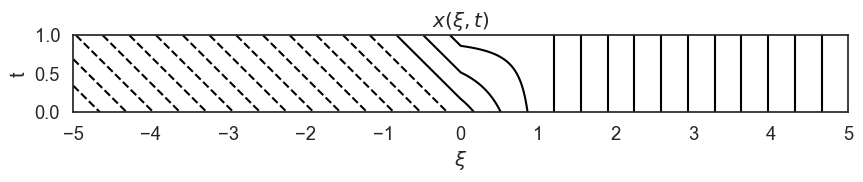
\includegraphics[width=\textwidth]{Fig1.png}
        \caption{Plot of $x(\xi, t)$}
        \label{fig:fig1}
      \end{figure}      

      We now invert $x(\xi, t)$ to find $\xi(x,t)$. Since we are restricting ourselves to the pre-shock domain $t < 1$, it is straightforward to invert the above expression to give us

      $$\xi(x,t) = \begin{cases} 
        x -t & x \le t \\
        \frac{x-t}{1-t} & t < x < 1 \\
        x & x \ge 1
      \end{cases}$$

      Using this expression, we may write our solution as 

      $$u(x,t) = u_0(\xi(x,t)) = \begin{cases}
        1 & \xi(x,t) \le 0 \\
        1-\xi(x,t) & 0 < \xi(x,t) < 1\\
        0 & \xi(x,t) \ge 1
      \end{cases}$$

      which we have plotted in Figure 2. 

      \begin{figure}[h]
        \centering
        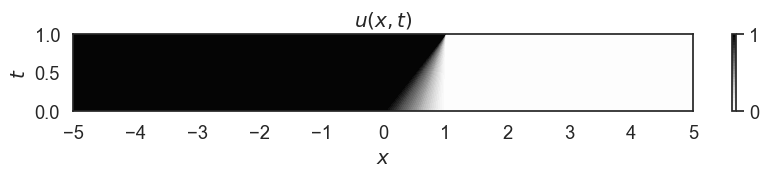
\includegraphics[width=\textwidth]{Fig2.png}
        \caption{Plot of $u(x, t)$ for $t < 1$}
        \label{fig:fig2}
      \end{figure}  
      
      \item In part (a) we determined the location of shock formation. To find the speed of the shock we can use the Rankine-Hugoniot condition. We first note that we can write our PDE in the form 
      
      $$\frac{\partial}{\partial t} u + \frac{\partial}{\partial x}\frac{1}{2} u^2 = 0$$

      which we recognize to be the conservation law form $f_t + g_x = 0$, where $u$ is a conserved density and $\frac{1}{2}u^2$ is its flux. We may write this conservation law in integral form over a small region $[x_1, x_2] = [\mathcal X -\epsilon, \mathcal X + \epsilon]$ which contains the location of the shock $\mathcal X(t)$. Let $u_1$ and $u_2$ denote the value of $u(x,t)$ on either side of the shock.

      $$\frac{d}{dt} \int_{x_1}^{x_2} u dx = -\frac{1}{2}(u_2^2- u_1^2)$$

      Now, splitting this integral up at $\mathcal X(t)$, we have 

      \begin{align*}
        \frac{d}{dt} \int_{x_1}^{\mathcal X} u dx + \frac{d}{dt} \int_{\mathcal X}^{x_2} u dx &= -\frac{1}{2}(u_2^2- u_1^2)\\
        \dot{\mathcal X} u_1 - \dot{\mathcal X} u_2 &= -\frac{1}{2}(u_2^2- u_1^2)
      \end{align*}

      and finally we have the shock speed 

      $$\dot{\mathcal X} = \frac{1}{2} \frac{u_2^2 - u_1^2}{u_2-u_1} = \frac{1}{2} (u_1 + u_2)$$

      For our PDE, we have $u_1 = 1$ and $u_2 = 0$, hence we have a shock speed of 

      $$\dot{\mathcal X} = \frac{1}{2}$$

      \item In part (b) we found the solution for $t < t^*=1$. For $t > 1$ the solution has a shock discontinuity which moves at constant speed $\dot x(t) = \frac{1}{2}$ beginning at the point $(1,1)$. All points to the left of the shock have value $1$, and all values to the right of the shock have value $0$, as the characteristic curves on either side meet at the shock. See Figure 3. 
      
      \begin{figure}[h]
        \centering
        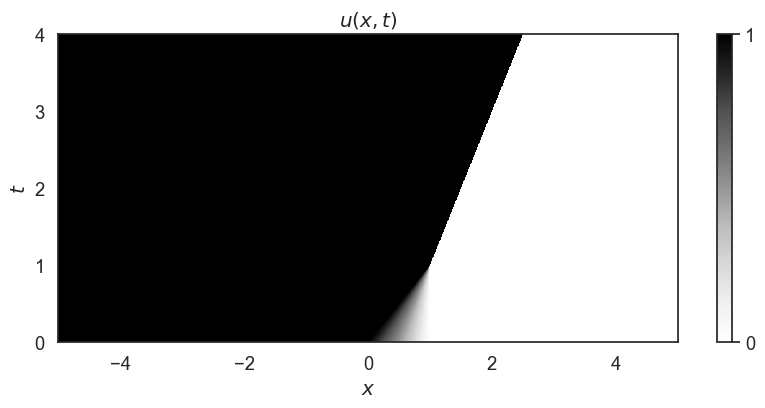
\includegraphics[width=\textwidth]{Fig3.png}
        \caption{Full plot of $u(x, t)$}
        \label{fig:fig3}
      \end{figure}  

    \end{enumerate}
  \end{solution}
  
  \begin{problem}
    Solve the PDE:
    \begin{align*}
        u_t + uu_x = u && -\infty < x < \infty  && t>0
    \end{align*}

    subject to the initial condition 
    \begin{align*}
        u(x,0)=u_0(x)=2x && 0 \le x \le 2
    \end{align*}

    Where in the x-t plane is the solution valid?
  \end{problem}
  \begin{solution}
    This is Burgers equation with dissipation. As above, its characteristics are given by 
    
    $$\dot x = u$$

    However due to the dissipation term this PDE is no longer homogeneous, and hence the solution along this curve must satisfy 

    \begin{align*}
      \dot u = u && \Rightarrow && u= u_0(\xi)\exp(t)
    \end{align*}

    Combining this with the first equation, we have 

    \begin{align*}
      \dot x = u_0(\xi) \exp(t) && \Rightarrow && x = u_0(\xi)\exp(t) -u_0(\xi) + \xi
    \end{align*}

    We now use our initial condition.

    $$x = 2\xi \exp(t) - 2\xi + \xi = 2 \xi \exp(t)- \xi$$

    Rearranging this, we solve for $\xi(x,t)$ 

    $$\xi(x,t) = \frac{x}{2\exp(t) -1}$$

    Our solution is therefore given by 

    $$u(x,t) = u_0(\xi(x,t))\exp(t) = \frac{2x \exp(t)}{2\exp(t)-1}$$

    Note that as our initial condition was specified only for $x \in [0,2]$ it follows that our result is valid only for $\xi(x,t) \in [0,2]$. This corresponds to a region bounded by $x=0$ and $x(t) = 4 \exp(t) -2$, inside of which our solution is valid. Hence, our final solution is given by:

    \begin{align*}
      u(x,t) = \frac{2x \exp(t)}{2\exp(t)-1} && 0 \le x \le 4 \exp(t) -2 && t>0
    \end{align*}

    See Figure 4 for a plot of this solution in its domain. 

    \begin{figure}[h]
      \centering
      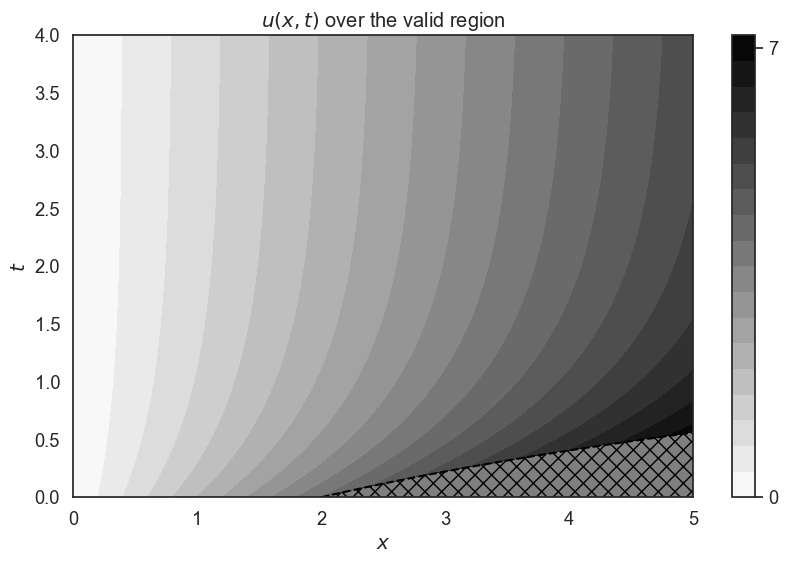
\includegraphics[width=\textwidth]{Fig4.png}
      \caption{Plot of $u(x, t)$ for $0 \le x \le 4 \exp(t) -2$ and $t>0$.}
      \label{fig:fig4}
    \end{figure}  

  \end{solution}

\end{document}
